%! TEX root = ../main.tex
\documentclass[../main.tex]{subfiles}

\begin{document}

\section{Rumore}

È stato notato come il rumore subisca una notevole variazione cambiando il fondoscala.

\begin{figure}[ht!]
    \centering
    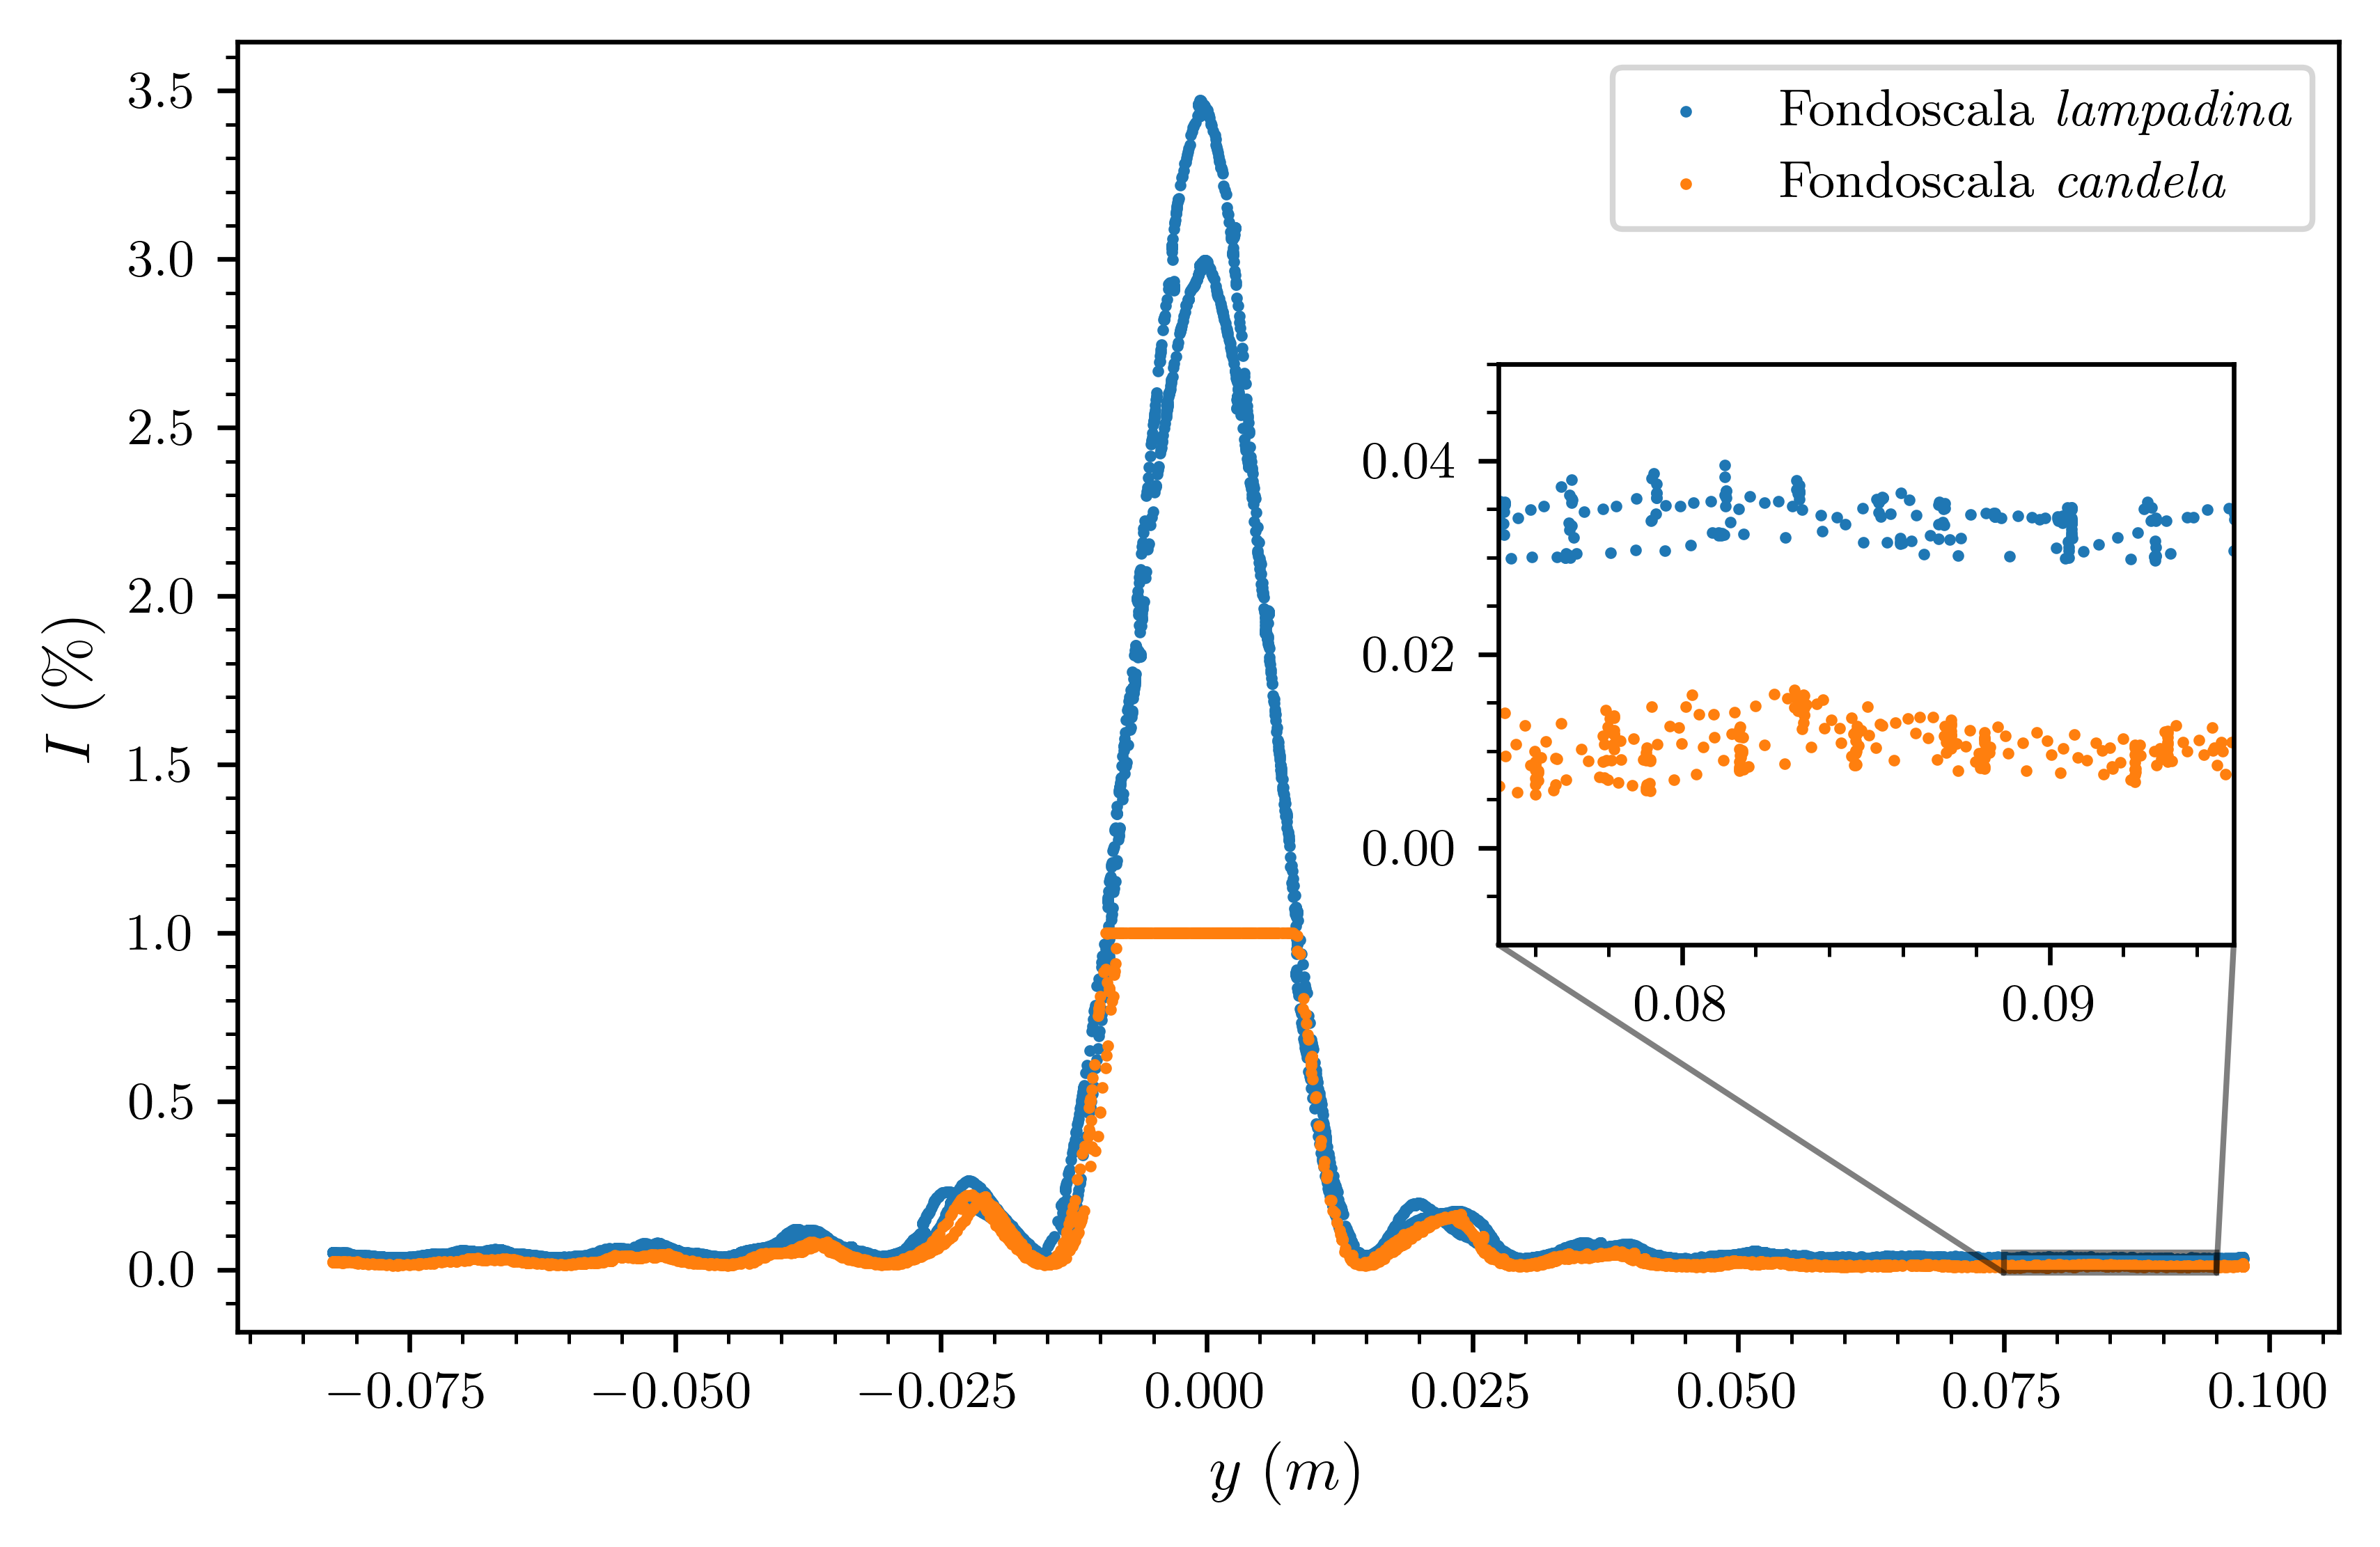
\includegraphics{scale_0.04.png}
    \caption{Grafico dell'intensità luminosa relativa $I$ in funzione della posizione $y$ (in metri) con apertura del sensore fissata a \qty{1.0}{\mm} e variando il fondoscala. È possibile osservare come il rumore registrato all'estremo della curva sia minore quando si utilizza un fondoscala differente, questo è stato attribuito alla variazione della corrente di buio per i diversi fondoscala che risulta essere \num{0.030+-0.006} per il fondoscala \textit{lampadina} e \num{0.017+-0.005} per il fondoscala \textit{candela}.} %? review: magari aggiungendo come sono state ricavate le misure della corrente di buio e come sono stati stimati gli errori su di esse (come semi-disperione delle misure più grande e più piccola)
\end{figure}

\end{document}